\documentclass[11pt]{amsart}
\usepackage{geometry}                % See geometry.pdf to learn the layout options. There are lots.
\geometry{letterpaper}                   % ... or a4paper or a5paper or ... 
%\geometry{landscape}                % Activate for for rotated page geometry
%\usepackage[parfill]{parskip}    % Activate to begin paragraphs with an empty line rather than an indent
\usepackage{graphicx}
\usepackage{amssymb}
\usepackage{epstopdf}
\usepackage{subfig}
\DeclareGraphicsRule{.tif}{png}{.png}{`convert #1 `dirname #1`/`basename #1 .tif`.png}
\bibliographystyle{abbrv}

\title{Evolution of internet information consumption through bookmarking}
\author{Kevin Leung}
%\date{}                                           % Activate to display a given date or no date

\begin{document}
\maketitle
As internet usage has grown recently, it has become important in our lives and has affected the way that we act and think. Particularly, people today consume and produce large amounts of media on the internet and in ways very different from before. A common complaint about this change, however, is that we experience information overload, with status updates constantly coming in from social networks, such as Twitter or Facebook, in small bursts relating to minor events. Some claim that there's a cost to this continuous flow of relatively unimportant information: we no longer pay attention to the big ideas or big movements in the world because we're stuck in the minutia \cite{big-idea} \cite{egypt}. 

For this project, we look at information consumption on the internet through social bookmarking usage over time to understand how people's attention and behavior has changed with the internet. We examine the number and age of bookmarks to particular URLs to understand the properties of usage. We also present an extension to preferential attachment that attempts to account for the time-sensitive nature of bookmarks.

\section{Related Work}
Kleinberg \cite{bursty-original} describes information streams as having bursty behavior, where individual events grow and disappear quickly. Kumar et al. \cite{bursty} applied this behavior specifically to the blogosphere. They looked at the evolution of the blogosphere into small communities and characterized its bursty behavior. Their time graph was able to also track the evolution of the network and look at when bursts happen. 

Gruhl et al. \cite{gruhl} looked specifically at how information spread through the blogosphere. By focusing on specific topics, they distinguished between the regular, long-running "chatter" around certain topics versus a "spike" from specific events. They also focus in on individuals to see how they behaved.

Leskovec et al. \cite{cascade} looked at cascades that occurred in the blogosphere. They discovered that most cascades are small, and these tended to be more wide than deep. In contrast to the last paper, however, they did not find bursty behavior across the blogosphere. Additionally, they also propose the \textit{Cascade generation model} to model the data they found.

Dorogovtsev and Mendes \cite{aging} extend the Barab\'{a}si-Albert preferential attachment \cite{barabasi} model to account for the age of the nodes in the network as well. Using the intuition that citations tend to prefer more recent publications, they show how the parameters and structure of networks change when attachment is proportional to the age of a node instead of its degree.

\section{Data Collection}
We used data from Delicious, a social bookmarking site, for this project. Since we're interested in the long-term evolution of behavior and long-range effects, it was important to have a dataset spanning several years, with the source of the bookmark as well as the time of the bookmark. G\"orlitz et al. \cite{goerlitz} has a corpus\footnote{https://www.uni-koblenz.de/FB4/Institutes/IFI/AGStaab/Research/DataSets/PINTSExperimentsDataSets/} with about 70 million bookmarks spanning from January 2003 through December 2006. The data included the date of the bookmark, the tags associated with the bookmark (which were discarded), an identifier for the bookmark target URL, and an identifier for the user. Unfortunately, because the URL itself wasn't included, we were unable to find any further information about the webpages, such as the type (commercial, blog, etc.) or the original time of creation. Particularly, the first bookmark associated with each node is treated as the beginning of that URL, though it might be long after the actual webpage was created.

To compare activity over time efficiently, we split the graph into 4 segments, each corresponding to a year. Between each year, the number of bookmarks increased significantly, jumping by an order of magnitude for the first 3 years:

\vspace{10pt}

\begin{tabular}{| l | l |}
 \hline
Year & Bookmark Count \\ \hline
2003 & 106549\\ \hline
2004 & 1833989 \\ \hline
2005 & 16120787 \\ \hline
2006 & 54627807 \\ \hline
\end{tabular}

\vspace{10pt}

One consequence of splitting these bookmarks by year is that some URLs may be split across years and treated as 2 separate cascades. Since the data doesn't exist before 2003 and isn't in the dataset after 2006, this scheme consistently evaluates each year and is an assumption used in previous research \cite{bursty-original}.

\section{Statistical Observations}
\subsection{Degree Analysis}
Initial analysis focused on large-scale changes from year to year to understand the general properties of the data. Although the number of bookmarks increased from year to year, it's also possible that the network scaled perfectly with it. First, we looked at the degree distribution over the bookmarks for particular target URLs, plotted in Figure 1 on a log-log scale.

\begin{figure}
	\centering
	\subfloat[]{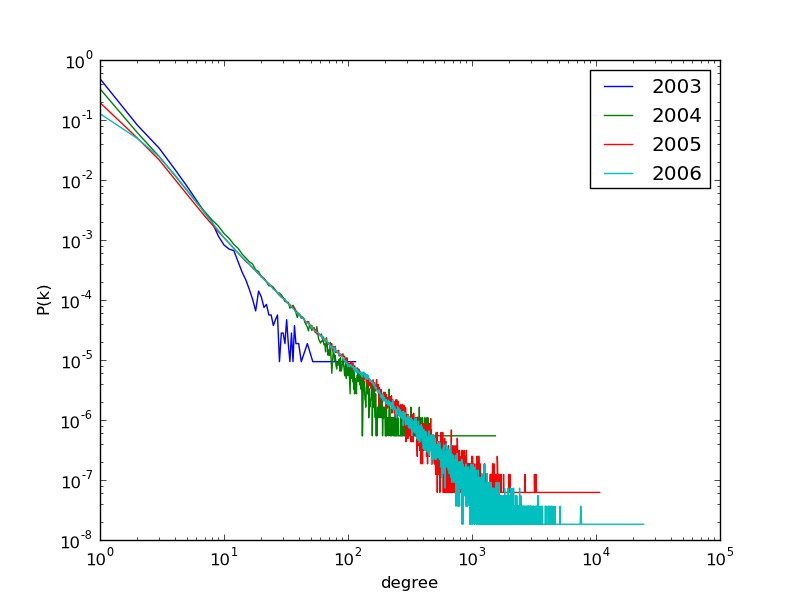
\includegraphics[width=4in]{degree_dist_p.png}}
	\subfloat[]{\begin{tabular}{| l | l | l |} \hline
		Year & Regression $\gamma$ & MLE $\gamma$ \\ \hline
		2003 & 2.75 & 5.00 \\ \hline
		2004 & 2.00 & 4.03\\ \hline
		2005 & 1.71 & 3.26\\ \hline
		2006 & 1.66 & 2.70 \\ \hline
		\end{tabular}
}
\caption{(A) shows the frequency of bookmark counts. (B) shows the estimated $\gamma$ using different methods.}
\end{figure}

The linear relationship on this scale suggests that it follows a power law distribution, $P(k) \propto k^{-\gamma}$.\footnote{I follow the convention of Dorogovtsev and Mendes \cite{aging} of assigning $\gamma$ the power law exponent. $\alpha$ will be used as the aging exponent.} The power law relationship intuitively make sense: many pages will only be bookmarked once, with larger counts being less likely. Interestingly, the estimated $\gamma$ also appears to be decreasing from year to year, which is somewhat inconsistent with the largely very similar appearance of the graphs. The difference appears to come towards the tail end of each distribution, where the sparsity of data may play a significant role.

The two methods of estimating $\gamma$ from the data yield vastly different results. Although MLE has been suggested to be a more accurate measure, the exponents are also significantly higher and beyond the range that we reasonably expect it to be. Particularly, $\gamma = 5$ would presumably require significantly more data to correctly estimate the expected number of nodes at the top end. Ironically, the higher $\gamma$s appear with less data in the earlier years. 

In qualitatively comparing the data against synthetic networks generated from the estimated $\gamma$s, the lower $\gamma$ estimates appear to be more correct. Although the power law relation should account for it, I can only guess that some extreme outliers with large bookmark counts are affecting the accuracy of these estimates.

\subsection{Bookmark Age Observations}
Past the number of bookmarks per URL, we're also interested in the frequency of bookmarking over time. Presumably, most bookmarks are made soon after the URL is first viewed, and the frequency decreases over time. To what degree this decrease happens, however, may change between years. To quantify this, we looked at the age of bookmarks, which is defined as the number of days that a bookmark appears after the first bookmark for that URL.

First, we looked the average age of bookmarks split by the total number of bookmarks for that URL. For comparison, we generated a random network inspired by the \textit{randomized Blogspace} model, which randomly shuffled the endpoint of every link in a blog network (similar to an Erd\H{o}s-R\'{e}nyi random graph) \cite{bursty}. Our model randomized the times of all of the bookmarks, which should evenly distribute the time overs all of the nodes and eliminate bursty behavior. We did, however, fix the degrees of the URLs, so the degree distribution remains the same. Figure 2 compares of the age of bookmarks versus degree for the actual and random graphs.

\begin{figure}
	\centering
	\subfloat[]{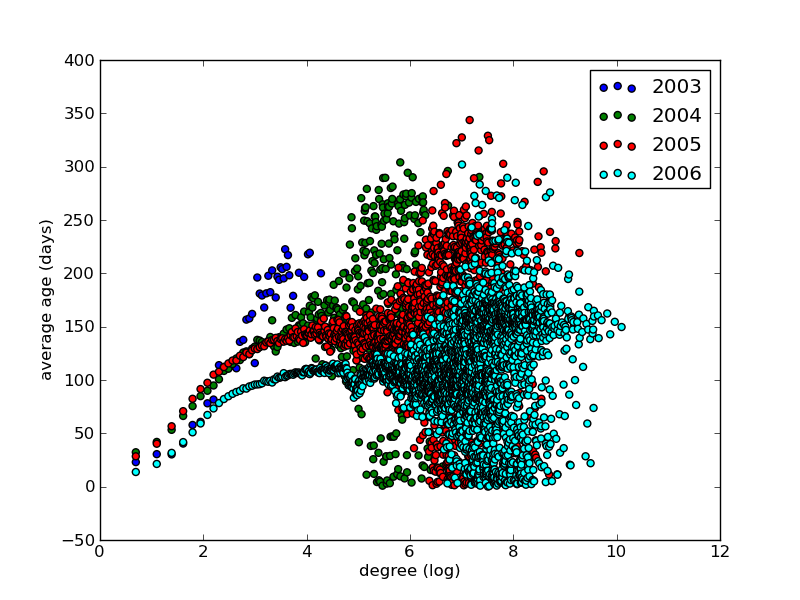
\includegraphics[width=3in]{time_plot.png}}
	\subfloat[]{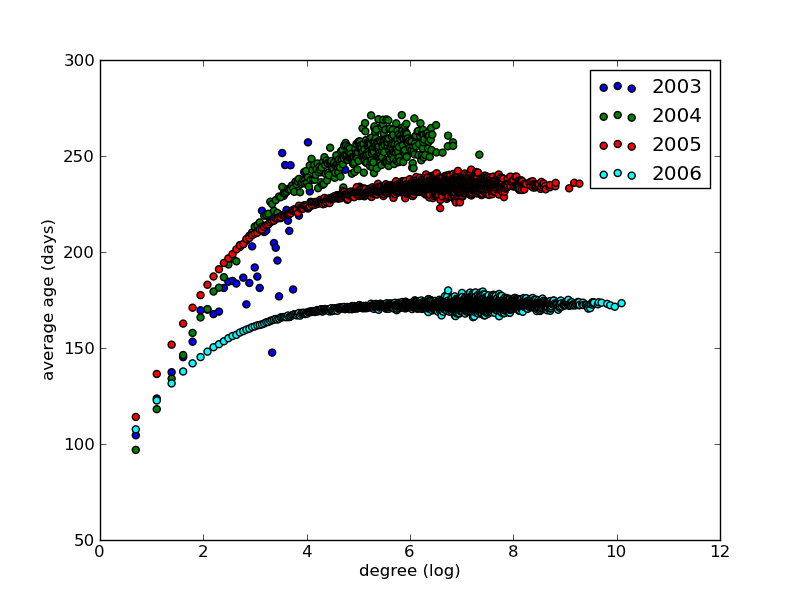
\includegraphics[width=3in]{time_plot_random.png}} \\
	\subfloat[]{\begin{tabular}{| l | l | l |} \hline
		Year & Network Average & Random Average \\ \hline
		2003 & 32.3 & 120.87\\ \hline
		2004 & 50.3 & 122.66 \\ \hline
		2005 & 50.79 & 139.58 \\ \hline
		2006 & 30.47 & 123.58 \\ \hline
		\end{tabular}
}
\caption{(A) shows the average age in the actual data, and (B) shows the same in the random graphs.}
\end{figure}

Interestingly, there's a drop in the average age over the years in both the real and random data. I immediately don't have an explanation for this result, though my intuition is that it could be related to the year-end truncation of data and the process of "filling in" the details as the network grows. This data also has very high variance in the average age for different URLs with the same degree. In the case of a URL bookmarked only twice, having one bookmark in January and one in December had a huge effect in increasing the average.

The network average time difference is significantly lower than that of the random network average time difference. This confirms our belief that most activity tends to happen early and around the same time instead of being distributed across the year. Otherwise, there is no pattern in this data.

Although the average age over bookmark degree provides an intuitive sense of total behavior, it doesn't immediately lend itself to a generative process or help us understand the bookmarks individually. To address this, we next looked at the age distribution in Figure 3.

\begin{figure}
	\centering
	\subfloat[]{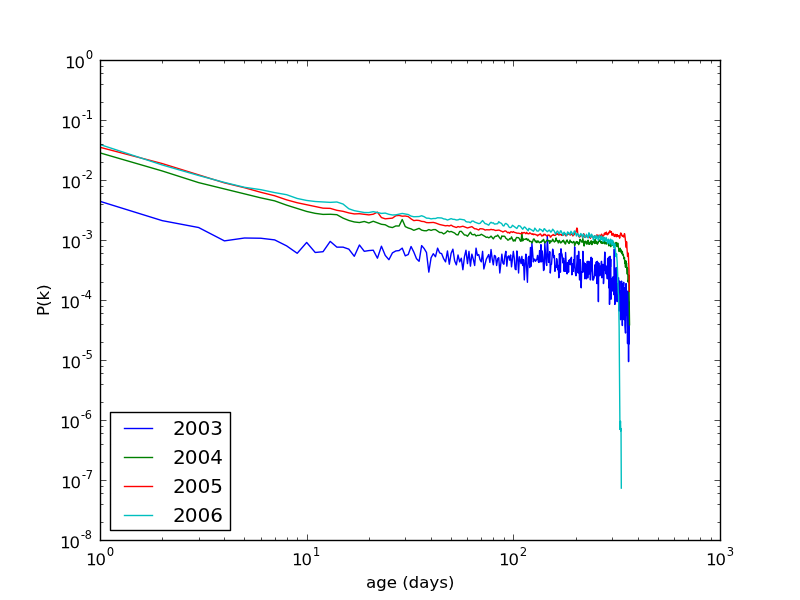
\includegraphics[width=3in]{delay_plot_p.png}}
	\subfloat[]{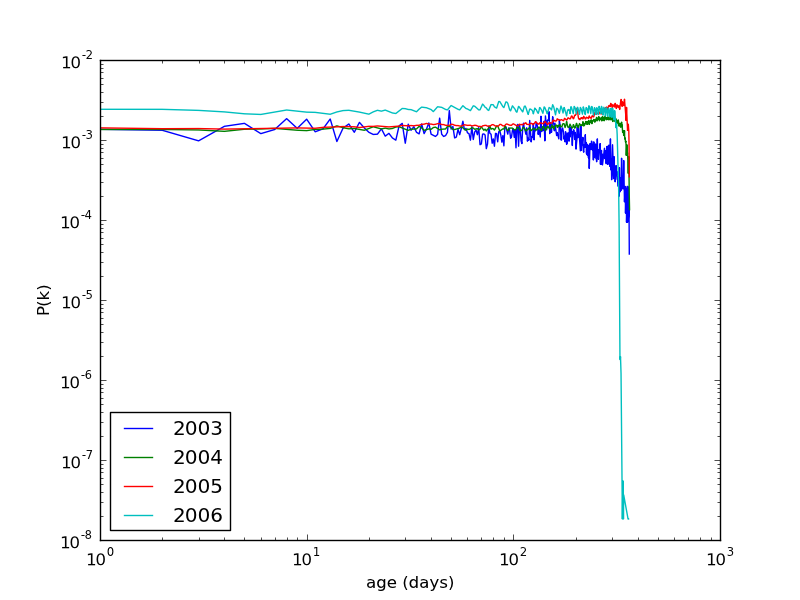
\includegraphics[width=3in]{delay_plot_p_random.png}}
\caption{(A) shows the age distribution in the actual data, and (B) shows the same in the random graphs.}
\end{figure}

From this, we can see that 2004 through 2006 all look very similar, while 2003 is somewhat different. On a log-log scale, the lines appear to be decreasing roughly linearly until nearing the maximum of 365 days in a year. This result demonstrates that from year to year, the proportion of the initial bookmarking remained relatively steady and decreased similarly over time.

One reason why 2003 might be different is that Delicious was started in 2003. Early behavior on the site might have differed significantly. A disproportionate amount of usage could have come from a small set of people, including Delicious employees and their friends and families. It's also possible that users hadn't developed a complete understanding how how to use Delicious. At the very least, there is significantly less data for 2003 to draw conclusions from.

The random graph also shows the results that we might expect: if we assume that the bookmark dates are roughly uniform, then the random shuffling should make any difference equally likely, until the cutoff of the duration of a year.

\section{Aging Model}

As is, the degree distribution can be modeled using the Barab\'{a}si-Albert preferential attachment \cite{barabasi} model. Unfortunately, this may provide a poor fit for the age of the bookmarks. Although users gravitate towards popular bookmarks, they also have a sense of time and will bookmark more recent content, as we saw in Figure 3. Dorogovtsev and Mendes \cite{aging} extend this model for age, but their model treats age as the timestep that a node is added in preferential attachment. Although we could use this notion of age, we also lack the specific ordering on a particular day and have so far been interested more in aggregating the data by day.

The simplest extension to this model is to simply replace the timestep with age in the attachment formula. The original aging model only has the preference dependent upon time, but we compare 3 different models, being standard preferential attachment, the aging model, and both of these combined for the following 3 models:

\begin{equation} P(k) \propto k^{-\gamma} \label{eq:pa}\end{equation}
\begin{equation} P(k) \propto \tau^{-\alpha} \label{eq:aging}\end{equation}
\begin{equation} P(k) \propto k^{-\gamma}\tau^{-\alpha} \label{eq:combined}\end{equation}

where $\tau$ is the number of days since the first bookmark + 1 (to avoid 0s in our equation).

To evaluate these models, we performed a grid search over possible parameter settings and took the least-squares log error of the model against the actual data on both the degree and age distribution. The best results were picked as those that minimized the sum of these two errors.

\subsection{Results}

Figure 4 shows the results on the 2003 data, and the table below shows the parameters of the best models for 2003. 

\begin{figure}
	\centering
	\subfloat[]{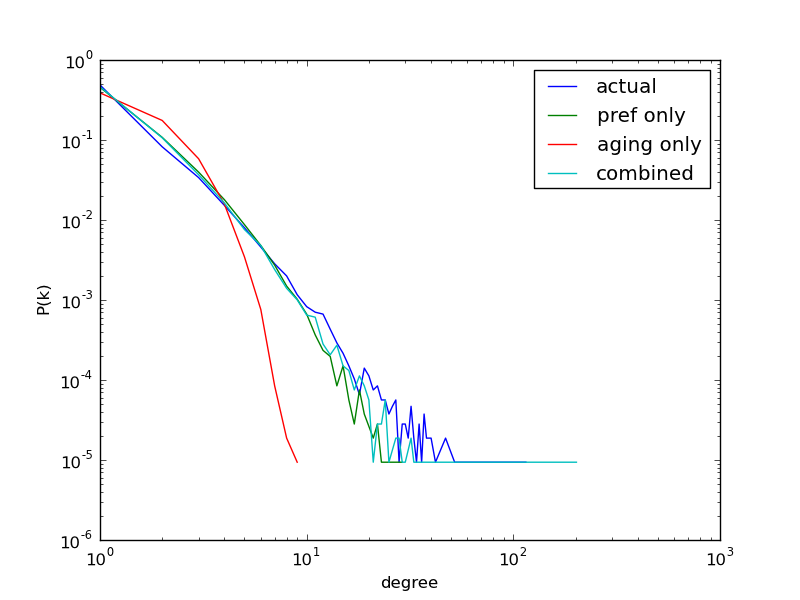
\includegraphics[width=3in]{aging_combined_2003.png}}
	\subfloat[]{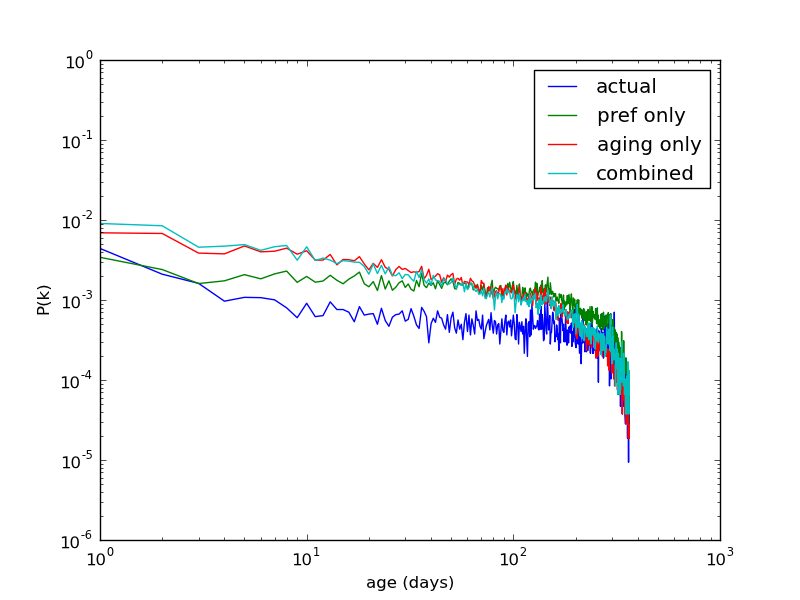
\includegraphics[width=3in]{aging_combined_delay_2003.png}} \\
\caption{(A) 2003 degree distribution, (B) 2003 age distribution}
\end{figure}

\vspace{10pt}
\begin{tabular}{| l | l | l | l | l |}
 \hline
2003 Model & Parameters & Degree Error & Age Error & Combined Error \\ \hline
pref only (1) & $\gamma = 1$ & 42.96 & 331.15 & 374.11 \\ \hline
aging only (2) & $\alpha = .25$ & 220.41 & 284.29 & 504.70 \\ \hline
combined (3) & $\gamma = 1.45, \alpha=.5$ & 18.430 & 243.68 & 262.11 \\ \hline
\end{tabular}
\vspace{10pt}

From the results for 2003, we can see that the combined model (3) provides a better fit for both the degree and age distribution than either model does independently. Although preferential attachment (1) appears to be closer to the actual data in the age distribution, it remains higher at the extreme values to the right, where the combined model (3) fits these cases better.

Although Dorogovtsev and Mendes \cite{aging} used this model to explain how they can maintain a scale-free distribution when $0 \leq \alpha \leq 1$, our aging model (2) showed no effect from $\alpha$ other than a large increase in error at extreme values. Otherwise, its error remained about the same as when $\alpha=0$ i.e. without any aging. This result may be an artifact of the bucketing process that we're doing by using days instead of time steps. Regardless, it is clear that this model needs to be coupled with preferential attachment to match the distribution.

\vspace{10pt}
\begin{tabular}{| l | l | l | l | l |}
 \hline
2004 Model & Parameters & Degree Error & Age Error & Combined Error \\ \hline
pref only (1) & $\gamma = 1.2 $ & 153.32 & 122.54 & 275.87 \\ \hline
aging only (2) & $\alpha = 0 $ & 1882.95 & 277.07 & 2160.02 \\ \hline
combined (3) & $\gamma = 1.2, \alpha=0$ & 153.32 & 122.54 & 275.87 \\ \hline
\end{tabular}
\vspace{10pt}

On the 2004 data, the best result came without the additional benefit of the aging variable. Even so, results were consistent within a range of $\alpha$ values, with increasing values trading off accuracy on the degree distribution for accuracy on the age distribution, until $\gamma=1.25, \alpha=.2$ with a combined error of 289.87. This result, however, is within a reasonable variance of the optimal value found based on other results since the model is random.

\begin{figure}
	\centering
	\subfloat[]{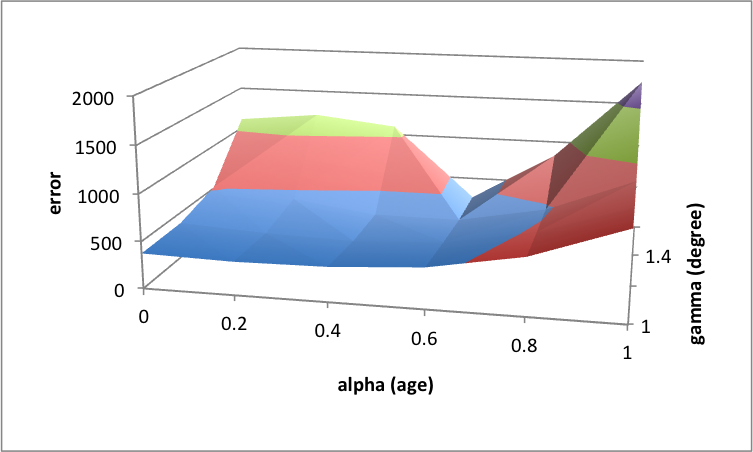
\includegraphics[]{modelerror2003.png}}
	\\
	\subfloat[]{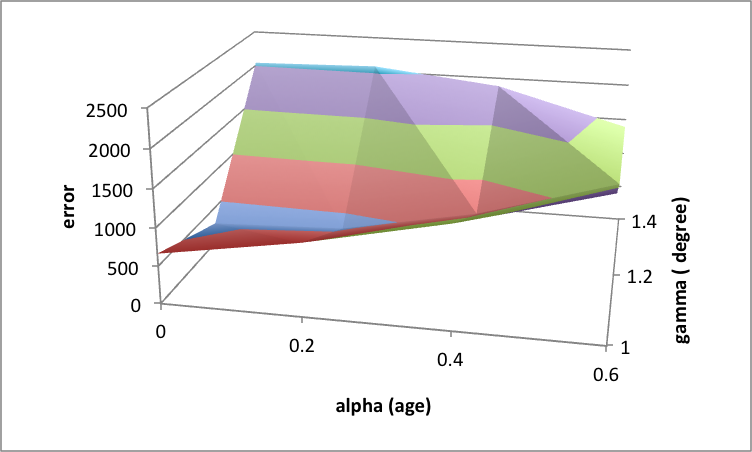
\includegraphics[]{modelerror2004.png}}
	\caption{(A) surface of the error with different values of $\alpha$ and $\gamma$ with (3) on 2003 (B) same for 2004}
\end{figure}

Figure 5 shows a surface of the error over the grid search within a small range around the optimal values. Although we were unable to derive a method of gradient descent, it appears that the surface is relatively smooth and should converge to an optimum. Although it may be difficult to see here, the data show that the error relatively low if the $\alpha and \gamma$ both increase linearly, and error only increases dramatically around this ravine.

Unfortunately, we were unable to apply the model to either the 2005 or 2006 data as they both proved to be intractable to compute (at least 1 week on the corn cluster). The 2003 model took approximately 5 minutes to compute, and the 2004 model took up to a day to compute. Given that 2005 data is an order of magnitude larger than 2004 and that the rate of growth is likely more than linear, this was unlikely to finish in the span of this project.

The main difficulty with running the combined model is computing the random assignment. Although preferential attachment has clever algorithms (such as randomly picking an edge) to avoid directly computing the probability of assignment to every node, these methods weren't helpful with (3) since $k$ and $\tau$ are multiplied directly to each other. 

\section{Discussion}
In summary, we looked at the age and frequency of bookmarks partitioned into years to understand how behavior has changed as the population has scaled by orders of magnitude of time. Looking at the degree distribution, we found that there was a power law relationship, and this was consistent from year to year. Looking at the average age for various degrees, we saw significant difference between years, but this was also correlated with the results from a randomized model, suggesting that this was an amplified effect of differences in the degree distribution. Looking at the age distribution, we again saw very consistent results in the proportion of bookmarks over time. Finally, we experimented with a model that combined the Barab\'{a}si-Albert preferential attachment model \cite{barabasi} and Dorogovtsev and Mendes aging model \cite{aging} and found that it was better able to fit the degree and age distribution.

Extrapolating back to our original question, we have 2 answers to the question about whether humans have been overloaded and narrowed by the explosion of information. First, the degree distribution and age distribution showed that the proportion of different bookmark popularity was largely consistent. Although the total usage and activity increased, the type of behavior appears to have scaled with the total number of Delicious users. Second, the combined model using both the degree and age of a previous target URL suggests that the prior popularity of a link and its recency are both important factors in how people attend to information on the internet.

\subsection{Future Work}

There are many opportunities for future work on this project. First, the model should be applied to larger models, and better methods for scaling with the data are needed to compute it. Even past this data, Delicious usage increased even more orders of magnitude since 2006, and it would be worthwhile to investigate behavior at the time as well. Deriving a method for gradient descent or more efficient multinomial selection may help here.

Second, this analysis was uninformed by any information about the social aspect of Delicious. Delicious is a social bookmarking service, and this adds significant complexity to the flow of information. It, however, is also an opportunity to gain more insight into the actual mechanisms of link discovery beyond preferential attachment.

Finally, this analysis didn't use the contents of the target URLs. One would expect that information would flow differently between communities and affect how particular URLs become popular. The target URLs also matter, as bookmarks can be used for many things. At one extreme are big services, such as Google, or reference pages that mostly have no time scale. At the other is microblogging, such as tweets or status updates, that are sensitive on the scale of minutes. There may be more subtle differences in behavior with respect to the type of content being bookmarked.

\bibliography{final}
\bibliographystyle{abbrv}

\end{document}  